\documentclass[12pt, twoside]{article}
\usepackage[letterpaper, margin=1in, head=30pt, headsep=0.1in]{geometry}
\usepackage[english]{babel}
\usepackage[utf8]{inputenc}
\usepackage{amsmath}
\usepackage{amsfonts}
\usepackage{amssymb}
\usepackage{tikz}
%\usetikzlibrary{quotes, angles}

\usepackage{graphicx}
\usepackage{enumitem}
\usepackage{multicol}

%\usepackage{pgfplots}
%\pgfplotsset{width=10cm,compat=1.9}
%\usepgfplotslibrary{statistics}
%\usepackage{pgfplotstable}
%\usepackage{tkz-fct}
%\usepackage{venndiagram}

\usepackage{fancyhdr}
\pagestyle{fancy}
\fancyhf{}
\renewcommand{\headrulewidth}{0pt} % disable the underline of the header
\raggedbottom

\title{Math AI Worksheet Generator and Formative Assessment System}
\author{Chris Huson}
\date{July 2018}

\fancyhead[RE]{\thepage}
\fancyhead[RO]{\thepage \\ Name: \hspace{3cm}}
%\fancyhead[L]{BECA / Dr. Huson / 10th Grade Geometry\\* 7 June 2019}
%
%\begin{document}
%\subsubsection*{13.7 Homework: Cross sections, distance applications}
\fancyhead[L]{BECA / Dr. Huson}

\begin{document}

\begin{enumerate}

\item Use symbols to write the name of each geometric figure.
    \begin{enumerate}
    \item %Ray DE
      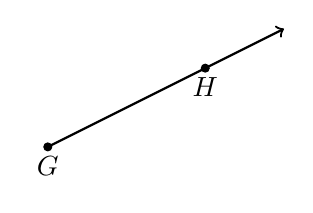
\begin{tikzpicture}
        \draw [->, thick] (0,0)--(3,1.5);
        \draw [fill] (0,0) circle [radius=0.05] node[below]{$G$};
        \draw [fill] (2,1) circle [radius=0.05] node[below]{$H$};
      \end{tikzpicture} \bigskip
    \item \hspace{1cm}%Line AB
      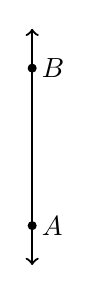
\begin{tikzpicture}
        \draw [<->, thick] (1,0)--(1,3);
        \draw [fill] (1,0.5) circle [radius=0.05] node[right]{$A$};
        \draw [fill] (1,2.5) circle [radius=0.05] node[right]{$B$};
      \end{tikzpicture} \bigskip
      \item %Line segment XY
        \begin{tikzpicture}
          \draw [-, thick] (1,0)--(0,2);
          \draw [fill] (1,0) circle [radius=0.05] node[below]{$E$};
          \draw [fill] (0,2) circle [radius=0.05] node[left]{$F$};
        \end{tikzpicture}
    \end{enumerate}


\item A flat surface is a(n) $\rule{4cm}{0.15mm}$. \bigskip


\item Find the value of $|2.5-3|$.


\item Two line segments or angles of equal measure are $\rule{4cm}{0.15mm}$.
      \bigskip


\end{enumerate}
\end{document}
